\chapter{Public-Data Transfer and Image-Only Deep Learning}\label{ch:5}

This chapter adds external knowledge: 4,827 ECG--echocardiography pairs from the public EchoNext data \cite{ref23}, redrawn in the hospital printout format. The EchoNext file was split by patient into 3,853 training and 974 locked EchoNext test ECGs.

\section{EchoNext in the printout format}\label{sec:5.1}

\begin{table}[htbp]
\caption{EchoNext-trained models: internal checks and transfer to the 837 hospital ECGs without any hospital training.}\label{tab:5.1}
\small
\begin{tabular}{>{\raggedright\arraybackslash\hspace{0pt}}p{\dimexpr 0.225\linewidth-2\tabcolsep\relax}%
>{\raggedright\arraybackslash\hspace{0pt}}p{\dimexpr 0.090\linewidth-2\tabcolsep\relax}%
>{\raggedright\arraybackslash\hspace{0pt}}p{\dimexpr 0.090\linewidth-2\tabcolsep\relax}%
>{\raggedright\arraybackslash\hspace{0pt}}p{\dimexpr 0.125\linewidth-2\tabcolsep\relax}%
>{\raggedright\arraybackslash\hspace{0pt}}p{\dimexpr 0.110\linewidth-2\tabcolsep\relax}%
>{\raggedright\arraybackslash\hspace{0pt}}p{\dimexpr 0.120\linewidth-2\tabcolsep\relax}%
>{\raggedright\arraybackslash\hspace{0pt}}p{\dimexpr 0.100\linewidth-2\tabcolsep\relax}%
>{\raggedright\arraybackslash\hspace{0pt}}p{\dimexpr 0.140\linewidth-2\tabcolsep\relax}}
\toprule
 & \multicolumn{2}{>{\raggedright\arraybackslash\hspace{0pt}}p{\dimexpr 0.180\linewidth-2\tabcolsep\relax}}{\textbf{EchoNext locked test (974)}}
 & \multicolumn{4}{>{\raggedright\arraybackslash\hspace{0pt}}p{\dimexpr 0.445\linewidth-2\tabcolsep\relax}}{\textbf{Hospital transfer AUROC / $\bm{r}$}}
 & \textbf{Zero-shot} \\
\cmidrule(lr){2-3}\cmidrule(lr){4-7}\cmidrule(lr){8-8}
\textbf{Model} & \textbf{Acc.} & \textbf{EF $\bm{r}$} & \textbf{EF$\bm{\le}$45} & \textbf{N vs Mi} & \textbf{Mi vs Mo} & \textbf{EF $\bm{r}$} & \textbf{4-class acc.} \\
\midrule
EN-cls (plan, ECGFounder embeddings) & 0.586 & 0.603 & 0.835 & 0.755 & 0.619 & 0.616 & 0.513 \\
EN-all, harmonised hospital input & 0.648 & 0.629 & \textbf{0.846} & \textbf{0.768} & 0.615 & \textbf{0.622} & 0.554 \\
EN-all, plain hospital input & -- & -- & 0.836 & 0.760 & 0.609 & 0.620 & \textbf{0.560} \\
\bottomrule
\end{tabular}
\end{table}


EchoNext waveforms were converted back to millivolts, resampled to 500 Hz, harmonised to the hospital baseline and cut into the printout's 2.5-s windows. The converted signals behave like the hospital's: heart-rate agreement $r=0.96$, QRS duration 82 against 82 ms and QTc 415 against 416 ms. Models trained only on EchoNext were then applied to the hospital printouts. \textbf{Transfer result.} Without any hospital training of the model, the EchoNext-trained classifier

separates EF $\le45$ \% from higher EF with AUROC \textbf{0.846}, Normal from Mild with 0.768, and estimates EF with $ r=0.62$. With only its decision thresholds tuned on the hospital training folds it reaches 0.551 four-class accuracy.

\section{Pruned ensembles of all image-derived models}\label{sec:5.2}

\begin{table}[htbp]
\caption{All ensemble variants (837 ECGs, original labels, corrected 95 \% CI). Members are the mean kept per fold.}\label{tab:5.2}
\footnotesize\setlength{\tabcolsep}{4pt}
\begin{tabular}{>{\raggedright\arraybackslash\hspace{0pt}}p{\dimexpr 0.076\linewidth-2\tabcolsep\relax}>{\raggedright\arraybackslash\hspace{0pt}}p{\dimexpr 0.100\linewidth-2\tabcolsep\relax}>{\raggedright\arraybackslash\hspace{0pt}}p{\dimexpr 0.150\linewidth-2\tabcolsep\relax}>{\raggedright\arraybackslash\hspace{0pt}}p{\dimexpr 0.139\linewidth-2\tabcolsep\relax}>{\raggedright\arraybackslash\hspace{0pt}}p{\dimexpr 0.174\linewidth-2\tabcolsep\relax}>{\raggedright\arraybackslash\hspace{0pt}}p{\dimexpr 0.159\linewidth-2\tabcolsep\relax}>{\raggedright\arraybackslash\hspace{0pt}}p{\dimexpr 0.110\linewidth-2\tabcolsep\relax}>{\raggedright\arraybackslash\hspace{0pt}}p{\dimexpr 0.089\linewidth-2\tabcolsep\relax}}
\toprule
\textbf{Pool} & \textbf{Selection} & \textbf{Meta-learner} & \textbf{Members} & \textbf{Accuracy [95 \% CI]} & \textbf{Recall N / Mi / Mo / S} & \textbf{Macro-F1} & \textbf{Adm.} \\
\midrule
base & greedy & LR (SUPER) & 3.1 & 0.583 [0.540, 0.626] & 0.90 / 0.15 / 0.50 / 0.27 & 0.451 & yes \\
base & greedy & STAGED-4 & 3.1 & 0.581 [0.535, 0.627] & 0.89 / 0.17 / 0.50 / 0.25 & 0.450 & yes \\
base & greedy & ordinal & 3.1 & 0.578 [0.537, 0.620] & 0.89 / 0.17 / 0.49 / 0.28 & 0.450 & yes \\
base & TOP10 & LR & 10 & 0.577 [0.556, 0.598] & 0.88 / 0.15 / 0.52 / 0.26 & 0.447 & yes \\
base & TOP10 & STAGED-4 & 10 & 0.581 [0.555, 0.607] & 0.89 / 0.16 / 0.50 / 0.29 & 0.454 & yes \\
base & TOP10 & \textbf{ordinal} & 10 & \textbf{0.587 [0.565, 0.610]} & 0.89 / 0.17 / \textbf{0.52} / \textbf{0.31} & \textbf{0.467} & yes \\
X & greedy & LR & 3.4 & 0.575 [0.540, 0.611] & 0.89 / 0.16 / 0.48 / 0.25 & 0.442 & yes \\
X & greedy & STAGED-4 & 3.4 & 0.575 [0.541, 0.610] & 0.88 / 0.17 / 0.50 / 0.25 & 0.444 & yes \\
X & greedy & ordinal & 3.4 & 0.577 [0.545, 0.610] & 0.90 / 0.18 / 0.46 / 0.27 & 0.448 & yes \\
X & TOP10 & LR & 10 & 0.579 [0.556, 0.603] & 0.91 / 0.15 / 0.47 / 0.26 & 0.443 & no \\
X & TOP10 & \textbf{STAGED-4} & 10 & \textbf{0.585 [0.557, 0.613]} & 0.89 / \textbf{0.18} / 0.51 / 0.26 & 0.455 & yes \\
X & TOP10 & ordinal & 10 & 0.576 [0.552, 0.600] & 0.89 / 0.16 / 0.49 / 0.27 & 0.449 & yes \\
\midrule
\multicolumn{4}{>{\raggedright\arraybackslash\hspace{0pt}}p{\dimexpr 0.466\linewidth-2\tabcolsep\relax}}{C3 (Phase 5 selected model, reads the printed header)} & 0.562 [0.519, 0.605] & 0.85 / 0.18 / 0.46 / 0.34 & 0.449 & yes \\
\bottomrule
\end{tabular}
\end{table}


Twenty-one image-derived members were pooled: ECGFounder heads, the ENH and ULT members, tabular feature models, the EF band model and the EchoNext-trained models. Inside every training fold, members were selected either greedily (gain $\ge0.002$, at most 10 members) or as the ten best single members (TOP10), and combined by a logistic, staged (STAGED-4: Normal / middle / Severe, then Mild against Moderate) or ordinal (Frank--Hall) meta-learner (Table~\ref{tab:5.2}). The best ensemble, SUPER-TOP10 with the ordinal meta-learner, reaches \textbf{0.587} [0.565, 0.610] with all four classes detected; the staged ensemble reaches \textbf{0.585}.

\section{Additional features for Mild and Moderate}\label{sec:5.3}

Seventy-three further features targeted the Mild and Moderate classes: repolarisation heterogeneity (TCRT, T-wave morphology dispersion, T complexity, non-dipolar residuum), QT dispersion, the QT variability index and per-lead R amplitude ratios. The strongest single markers were TCRT (AUROC 0.738 for Normal against reduced EF) and the lead I R ratio (0.731). They were added as members of the extended ensemble pool (X), which gave the best staged model.

\section{Image-only pixel models with EchoNext pre-training}\label{sec:5.4}

\begin{figure}[htbp]
\centering
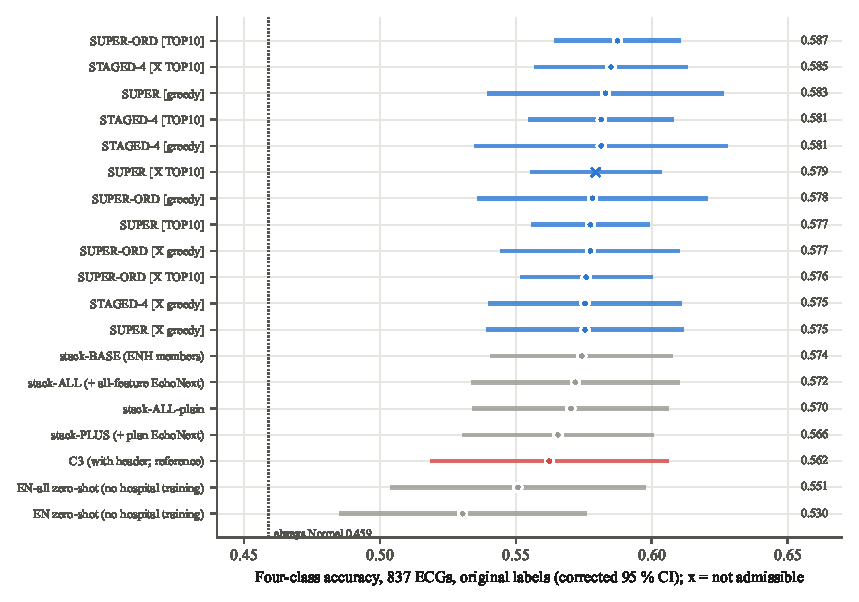
\includegraphics[width=0.91\linewidth,height=0.80\textheight,keepaspectratio]{figures/fig_5_1}
\caption{Four-class accuracy of every stack and ensemble variant of the public-data study, with cor- rected 95 \% confidence intervals.}\label{fig:5.1}
\end{figure}

\begin{table}[htbp]
\caption{Pixel models on the 837 hospital images (class weights tuned inside the training folds).}\label{tab:5.3}
\small
\begin{tabular}{>{\raggedright\arraybackslash\hspace{0pt}}p{\dimexpr 0.298\linewidth-2\tabcolsep\relax}>{\raggedright\arraybackslash\hspace{0pt}}p{\dimexpr 0.142\linewidth-2\tabcolsep\relax}>{\raggedright\arraybackslash\hspace{0pt}}p{\dimexpr 0.157\linewidth-2\tabcolsep\relax}>{\raggedright\arraybackslash\hspace{0pt}}p{\dimexpr 0.167\linewidth-2\tabcolsep\relax}>{\raggedright\arraybackslash\hspace{0pt}}p{\dimexpr 0.123\linewidth-2\tabcolsep\relax}>{\raggedright\arraybackslash\hspace{0pt}}p{\dimexpr 0.110\linewidth-2\tabcolsep\relax}}
\toprule
\textbf{Model} & \textbf{Accuracy [95 \% CI]} & \textbf{Recall N / Mi / Mo / S} & \textbf{Precision N / Mi / Mo / S} & \textbf{Macro-F1} & \textbf{Inner-val acc.} \\
\midrule
FT-IN: ResNet-18, ImageNet only & 0.492 [0.446, 0.537] & 0.75 / 0.20 / 0.36 / 0.24 & 0.69 / 0.23 / 0.37 / 0.25 & 0.386 & -- \\
ZS: ResNet-18, EchoNext only & 0.524 [0.493, 0.556] & 0.86 / 0.18 / 0.27 / 0.32 & 0.63 / 0.27 / 0.42 / 0.37 & 0.403 & -- \\
FT-EN: ResNet-18, EchoNext + fine-tuning & 0.530 [0.481, 0.578] & 0.82 / \textbf{0.23} / 0.34 / 0.29 & 0.71 / 0.29 / 0.38 / 0.29 & 0.416 & 0.569 \\
E2: ConvNeXt-T 384 $\times$ 768 & 0.535 [0.484, 0.586] & 0.80 / 0.22 / 0.40 / 0.31 & -- & \textbf{0.433} & 0.583 \\
E3: ConvNeXt-T, EF-led + EF grading & 0.540 [0.511, 0.570] & 0.86 / 0.17 / 0.35 / 0.34 & -- & 0.419 & 0.597 \\
E4: E3 + layer-wise LR, mixup, TTA, 3 seeds (final) & \textbf{0.548 [0.513, 0.582]} & 0.85 / 0.18 / 0.41 / 0.28 & -- & 0.423 & \textbf{0.604} \\
E6: triage on E4 (answers 60.6 \%) & 0.661 on answered & -- & -- & -- & -- \\
E5: stack-ALL + E3 network (pixels + traces) & 0.569 [0.534, 0.604] & 0.90 / 0.17 / 0.42 / 0.26 & -- & -- & -- \\
\bottomrule
\end{tabular}
\end{table}


Pixel CNNs read the page image directly. EchoNext ECGs were drawn as hospital printouts and used to pre-train them, before fine-tuning on the hospital images. Pre-training on the printoutformat EchoNext images raised ResNet-18 from 0.492 (ImageNet only) to 0.530. The final model, a three-seed ConvNeXt-Tiny ensemble trained with an EF-led loss, layer-wise learning rates, mixup and test-time augmentation, reached \textbf{0.548} [0.513, 0.582] from the page pixels alone (Table~\ref{tab:5.3}), within about two points of C3, which also reads the printed measurements. As a triage model it answers 60.6 \% of the ECGs at 0.661, and its 50 \% most confident ECGs are graded with 0.70 accuracy (descriptive). Added to the stacks, the pixel network gave 0.569.

